\documentclass[11pt]{amsart}

\usepackage{a4wide}
\usepackage{bbm}
\usepackage{graphicx}

\newcommand{\R}{\mathbbm{R}}

\title{Specification of the project\\``Orbits in Coxeter Groups''}
\author{Julian Pfeifle\\ Implementation of Geometric Algorithms, 2015}
\date{May, 2015}
\begin{document}

\maketitle

\section{Input}

The input to your program consists of 
\begin{itemize}
\item a string of length 2 of the form {\tt X}$n$, where {\tt X} is a letter and $n$ a number
\item A vector $v$ of length $n$
\end{itemize}

You should read this data from a file that contains the string on the first line and the vector on the second.

Your code for processing this data should be in a separate function that is called from the function responsible for reading the input. This also makes it possible to test your program from the testsuite.


\section{Validation}

\begin{itemize}
\item The input string must refer to a Coxeter arrangement of hyperplanes, i.e., be one of
  \begin{center}
    \ttfamily A$n$, B$n$, D$n$, E6, E7, E8, F4, G2, H3, H4, I$n$.

    \bigskip
    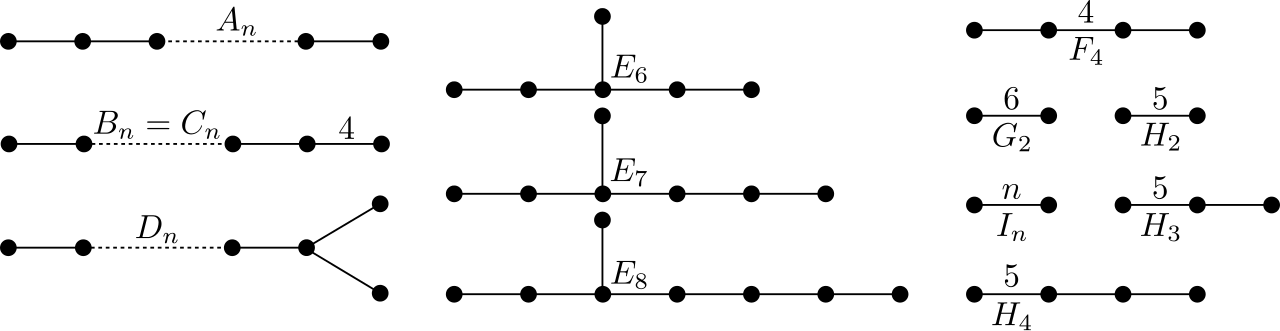
\includegraphics[width=\linewidth]{finite-coxeter.png}
  \end{center}
\item The vector $v$ should really have length $n$
\end{itemize}


\section{Processing}

\begin{enumerate}
\item First, you must determine a set of reflecting linear hyperplanes corresponding to the selected Coxeter group. These should be represented by their normal vectors, and these in turn should be hard-coded in your program.

For example, a standard set of normal vectors for the Coxeter arrangement of type~$A_n$ is formed by the rows of the matrix
\[
  \begin{pmatrix}
     1 & -1 &  0 & 0 &\dots &  0 &  0 \\
     0 &  1 & -1 & 0 &\dots &  0 &  0 \\
     \dots\\
     0 &  0 &  0 & 0 &\dots & -1 & 0 \\
     0 &  0 &  0 & 0 &\dots &  1 & -1
   \end{pmatrix},
\]
and for type $B_n$ by the rows of the matrix
\[
  \begin{pmatrix}
     1 & -1 &  0 & 0 &\dots & 0 & 0\\
     0 &  1 & -1 & 0 &\dots & 0 & 0\\
     \dots\\
     0 &  0 &  0 & 0 &\dots & 1 & -1\\
     0 &  0 &  0 & 0 &\dots & 0 & 1
   \end{pmatrix}.
\]
Notice that the matrix for $A_n$ has size $n\times(n+1)$, so it specifies $n$~normal vectors in $\R^{n+1}$. This is the only Coxeter group for which this happens, all the others (for example the group~$B_n$ in the second example) are generated by $n$~vectors in~$\R^n$. 

Also, you should check that the relation
\[
   \cos\frac{\pi}{p_{i,j}}
   \ = \
   -\frac{\langle w_i, \; w_j\rangle}{\|w_i\|\|w_j\|}
\]
holds for any pair of vectors $w_i$, $w_j$ of $A_n$ and $B_n$, where $\frac{\pi}{p_{i,j}}$ is the angle between the hyperplanes with normal vectors $w_i$~and~$w_j$, and $p_{i,j}$~is encoded by the Coxeter-Dynkin diagram: Two nodes not connected by an edge have $p_{i,j}=2$, an undecorated edge between two nodes represents $p_{i,j}=3$, and in all other cases the edge is labeled with $p_{i,j}$.

Can you find representative matrices for other Coxeter diagrams?
\end{enumerate}

\section{Output}

By default, you should output the size of the orbit of~$v$ that is obtained by repeatedly reflecting~$v$ in the hyperplanes given by the~$w_i$. Via a flag on the command line, you should be able to specify whether to additionally output the orbit itself.

\end{document}
